\documentclass[11pt,a4paper]{article}
\usepackage{gtu-el-yazisi}
\begin{document}
\notbilgi{Analog Haberleşme}{Fourier serisi açılımları ve spektrum}{Ders3.pdf}

\sayfa{1}
\section{Genelleştirilmiş Fourier Serisi Açılımı}
\textbf{Hatırlatma}

The signals $\psi_1(t),\ \psi_2(t),\ \ldots,\ \psi_N(t)$ ortagonal over $[t_1,t_2]$ if
\[ \int_{t_1}^{t_2}\psi_m(t)\,\psi_n^{*}(t)\,dt=\begin{cases} 0, & m\neq n \\ E_m, & m=n\end{cases} \]
In addition, if $E_m=1\ \forall m$ the signals are \underline{orthonormal}.

\medskip
Herhangi bir $x(t)$ işaretinin bu $N$ ortogonal (dik) işaret ile yaklaşımını elde edelim
\begin{align*}
x(t) &\cong c_1\psi_1(t)+c_2\psi_2(t)+\cdots+c_N\psi_N(t) \\
&= \sum_{n=1}c_n\psi_n(t),\quad t_1\le t\le t_2
\end{align*}
\begin{align*}
\text{Hata işareti (error signal)} &= e(t) = x(t)-\sum_{n=1}^{N}c_n\psi_n(t) \\
\text{Hatanın enerjisi (energy of error)} &= E_e = \int_{t_1}^{t_2}|e(t)|^2\,dt
\end{align*}
Eğer yaklaşımın katsayıları
\[ c_n=\frac{1}{E_n}\overbrace{\int_{t_1}^{t_2}x(t)\,\psi_n^{*}(t)\,dt}^{\text{korelasyon}};\quad n=1,\ldots,N \]
olarak seçilirse hatanın enerjisi minimum olur.

Ortagonal işaret kümesi tam (complete) ise hatanın enerjisi sıfıra gider ve yaklaşıklık eşitlik olur.
\[ x(t)=c_1\psi_1(t)+c_2\psi_2(t)+\cdots+c_N\psi_N(t)+\cdots=\sum_{n=1}^{\infty}c_n\psi_n(t),\quad t_1\le t\le t_2 \]
$\hookrightarrow$ Genelleştirilmiş F.S açılımı (Generalized FS expansion)

\sayfa{2}
\sekilnotu[2]{Bu sayfa tahtaya yazılmış notların fotoğrafıdır (eğik çekilmiş); içerik aşağıda aktarılmıştır.}
Eğer yaklaşımın katsayıları
\[ C_n=\frac{1}{E_n}\int_{t_1}^{t_2}x(t)\,\psi_n^{*}(t)\,dt\ ;\quad n=1,\ldots,N \]
olarak seçilirse hatanın enerjisi minimum olur.

Ortogonal işaret kümesi tam (complete) ise hatanın enerjisi sıfıra gider ve yaklaşıklık eşitlik olur:
\[ x(t)=C_1\psi_1(t)+C_2\psi_2(t)+\cdots+C_N\psi_N(t)+\cdots=\sum_{n=1}^{\infty}C_n\psi_n(t),\quad t_1\le t\le t_2 \]
$\hookrightarrow$ Genelleştirilmiş FS açılımı (Generalized FS expansion)

($x(t)$ işaret ailesi için $N\to\infty$ $E_e\to 0$ ise $\overbrace{\{\psi_n(t)\}}^{\text{Basis functions (Temel fonksiyonlar)}}$ ailesi tamdır. Bu durumda $x(t)$ işaret ailesi içindeki bütün işaretleri bu temel fonksiyonlar ile ifade etmek mümkündür.)

Parseval teoremi:
\[ E_x=C_1^2E_1+C_2^2E_2+\cdots+C_N^2E_N+\cdots=\sum_{n=1}^{\infty}C_n^2E_n \]

\sayfa{3}
\section{Trigonometrik FS açılımı}
$\forall t\ \ x(t+T_0)=x(t)$

F. Serisinin mevcut olma şartları:

1) $x(t)$ bir periyoda boyunca mutlak integrali alınabilir olmalıdır:
\[ \int_{T_0}|x(t)|\,dt<\infty \]
(fourier serisi vardır, her noktada yakınsamaya bilir) \hfill $\}$ Zayıf (weak) Dirichlet şartı

2) $x(t)$'nin bir periyodunda sonlu sayıda maksimumu, minimumu ve süreksizliği vardır. \hfill $\}$ Kuvvetli (strong) Dirichlet şartları

İkisi sağlanıyorsa fourier serisi açılımı vardır.

\textcolor{kirmizikalem}{$\ast$} Laboratuvarda üretilen işaretlerin fourier açılımı vardır

\[ x(t)=a_0+\sum_{n=1}^{\infty}\Big[a_n\cos(n\omega_0 t)+b_n\sin(n\omega_0 t)\Big] \qquad t_1\le t\le t_1+T_0 \]
\[ \omega_0=2\pi f_0=\frac{2\pi}{T_0} \]
\begin{align*}
a_0&=\frac{1}{T_0}\int_{T_0}x(t)\,dt, & a_n&=\frac{2}{T_0}\int_{T_0}x(t)\cos(n\omega_0 t)\,dt, & n&=1,2,\ldots \\
& & b_n&=\frac{2}{T_0}\int_{T_0}x(t)\sin(n\omega_0 t)\,dt, & n&=1,2,\ldots
\end{align*}
$x(t)$ tek $\Rightarrow a_0=a_n=0$

$x(t)$ çift $\Rightarrow b_n=0$

\formulkutu[ortogonal]{\begin{aligned}
  &\forall n,m\quad \int_{T_0}\sin(n\omega_0 t)\cos(m\omega_0 t)\,dt=0 \ \ \nearrow\ \text{ortagonaltir} \\[2mm]
  &\hphantom{\forall n,m\quad}\int_{T_0}\cos(n\omega_0 t)\cdot\cos(m\omega_0 t)\,dt=\begin{cases} 0 & n\neq m \\ T_0/2 & n=m\end{cases} \\[2mm]
  &\hphantom{\forall n,m\quad}\int_{T_0}\sin(n\omega_0 t)\,\sin(m\omega_0 t)\,dt=\begin{cases} 0, & n\neq m \\ T_0/2 & n=m\end{cases}
\end{aligned}}

\[ \text{Parseval teoremi}:\quad P_x=a_0^2+\frac{1}{2}\sum_{n=1}^{\infty}\left(a_n^2+b_n^2\right) \]

\sayfa{4}
\section{Compact FS Expansion}
\[ a_n\cos(n\omega_0 t)+b_n\sin(n\omega_0 t)=c_n\cos(n\omega_0 t+\theta_n) \]
\begin{align*}
c_n &= \sqrt{a_n^2+b_n^2}\ ,\qquad c_0=a_0 \\
\theta_n &= -\arctan\!\left(\frac{b_n}{a_n}\right) \\
x(t) &= c_0+\sum_{n=1}^{\infty}c_n\cdot\cos(n\omega_0 t+\theta_n) \qquad\qquad t_1\le t\le t_1+T_0
\end{align*}
\begin{align*}
&\text{Parseval Teoremi}:\quad P_x=c_0^2+\frac{1}{2}\sum_{n=1}^{\infty}c_n^2 \\
&\qquad\qquad\qquad\ \uparrow \\
&\text{Parseval teoremi}:\quad P_x=a_0^2+\frac{1}{2}\sum_{n=1}^{\infty}\left(a_n^2+b_n^2\right)
\end{align*}

\subsection{Fourier spektrumu}
\noindent
\begin{tabular}{@{}l@{\hspace{1.2cm}}l@{\hspace{3mm}}c@{\hspace{3mm}}l@{}}
  $c_n\times f=nf_0$ & Genlik (Amplitude) spektrumu & \multirow{2}{*}{$\left.\rule{0pt}{1.1cm}\right\}$} & \multirow{2}{*}{\shortstack[l]{Çizgi\\(Line)\\spektrum}} \\
  $\theta_n\times f=nf_0$ & Faz (Phase) \hspace{1.8cm} $''$ & & \\
\end{tabular}

\section{Üstel FS Expansion}
(Complex/Exponential FS expansion)
\begin{align*}
c_n\cos(n\omega_0 t+\theta_n) &= c_n\cdot\frac{1}{2}\Big[e^{j(n\omega_0 t+\theta_n)}+e^{-j(n\omega_0 t+\theta_n)}\Big] \\
&= \underbrace{\frac{1}{2}c_n e^{j\theta_n}}_{x_n}\cdot e^{jn\omega_0 t}+\underbrace{\frac{1}{2}c_n\cdot e^{-j\theta_n}}_{x_{-n}}e^{-jn\omega_0 t}
\end{align*}
\[ x(t)=\sum_{-\infty}^{\infty}x_n\,e^{jn\omega_0 t} \]
\[ x_n=\frac{1}{T_0}\int_{T_0}x(t)\,e^{-jn\omega_0 t}\,dt \]
\[ \int_{T_0}\underbrace{e^{jm\omega_0 t}\cdot e^{-jn\omega_0 t}}_{e^{j(m-n)\omega_0 t}}\,dt=\begin{cases} 0, & n\neq m \\ T_0, & n=m\end{cases} \]
\[ \text{Parseval teoremi}:\quad P_x=\sum_{n=-\infty}^{+\infty}|x_n|^2 \]
$e^{jn\omega_0 t}$ nin gücü 1 dir.

\sayfa{5}
\begin{align*}
x_n &= \frac{1}{2}c_n e^{j\theta_n} & n&=1,2,\ldots\infty \\
x_{-n} &= \frac{1}{2}c_n e^{-j\theta_n} & n&=1,2,\ldots\infty \\
x_0 &= c_0 = a_0
\end{align*}
\subsection{Üstel F. spektrumu}
\begin{align*}
x_n &= |x_n|\,e^{j\theta_n} \\
x_{-n} &= |x_n|\,e^{-j\theta_n} \\
|x_{-n}| &= |x_n| = \frac{1}{2}c_n \\
\angle x_n &= \theta_n, \qquad \angle x_{-n}=-\theta_n
\end{align*}
\noindent
\begin{tabular}{@{}l@{\hspace{1.5cm}}l@{}}
  $|x_n|\times f=nf_0$ & Genlik spektrumu \\
  $\angle x_n\times f=nf_0$ & Faz spektrumu
\end{tabular}

\begin{ornek}
  Find compact FS expansion of $x(t)$ \\
  (Unipolar square wave) \\
  Tek kutuplu kare dalgası
\end{ornek}
\begin{center}
  \begin{tikzpicture}
    \begin{axis}[width=14cm, height=3.2cm, xmin=-8.6, xmax=8.9, ymin=-0.35, ymax=1.5,
        xtick={-6.2832,-3.1416,-1.5708,1.5708,3.1416,6.2832},
        xticklabels={$-2\pi$,$-\pi$,$-\pi/2$,$\pi/2$,$\pi$,$2\pi$}, ytick=\empty]
      \addplot[kirmizikalem!55, line width=1.1pt] coordinates {(-7.854,0) (-7.854,1) (-4.712,1) (-4.712,0)};
      \addplot[kirmizikalem!55, line width=1.1pt] coordinates {(-1.5708,0) (-1.5708,1) (1.5708,1) (1.5708,0)};
      \addplot[kirmizikalem!55, line width=1.1pt] coordinates {(4.712,0) (4.712,1) (7.854,1) (7.854,0)};
    \end{axis}
  \end{tikzpicture}
\end{center}
$\Rightarrow T_0=2\pi$
\[ x(t)=a_0+\sum_{n=1}^{\infty}\Big[a_n\cos(n\omega_0 t)+b_n\sin(n\omega_0 t)\Big] \]
\begin{align*}
a_0 &= \frac{1}{T_0}\int_{T_0}x(t)\,dt = \frac{1}{2\pi}\int_{-T_0/2}^{T_0/2}x(t)\,dt = \frac{1}{2\pi}\int_{-\pi/2}^{\pi/2}1\,dt \\
&= \frac{1}{2\pi}\,\pi = \frac{1}{2} \qquad\qquad (\omega_0=1)
\end{align*}
\begin{align*}
a_n &= \frac{2}{T_0}\int_{T_0}x(t)\cdot\cos(nt)\,dt \qquad\qquad \omega_0=\frac{2\pi}{T_0}=\frac{2\pi}{2\pi}=1 \\
&= \frac{2}{2\pi}\int_{-\pi/2}^{\pi/2}1\cdot\cos(nt)\,dt=\frac{1}{\pi}\left.\frac{\sin(nt)}{n}\right|_{-\pi/2}^{+\pi/2}
\end{align*}

\sayfa{6}
\[ =\frac{1}{\pi n}\left[\sin\left(\frac{n\pi}{2}\right)-\sin\left(-\frac{n\pi}{2}\right)\right] \]
\[ a_n=\frac{2}{\pi n}\sin\left(\frac{n\pi}{2}\right)=\begin{cases} 0, & n\ \text{çift ise} \\[1mm] \dfrac{2\pi}{n}, & n=1,5,9 \\[2mm] -\dfrac{2\pi}{n}, & n=3,7,11 \end{cases}\text{\footnotemark} \]
\footnotetext{Claude notu: muhtemelen $\dfrac{2}{\pi n}$ ve $-\dfrac{2}{\pi n}$ olmalı.}
$x(t)$ çift $\Rightarrow b_n=0$

\formulkutu[ezberle]{\begin{aligned}
  x(t)&=\frac{1}{2}+\frac{2}{\pi}\Big[\cos(\omega_0 t)-\frac{1}{3}\cos(3\omega_0 t)+\frac{1}{5}\cos(5\omega_0 t) \\
  &\qquad\quad -\frac{1}{7}\cos(7\omega_0 t)+\cdots\Big]
\end{aligned}}
\formulkutu{-\cos a=\cos(a-\pi)}
\formulkutu[ezberle]{\begin{aligned}
  x(t)&=\frac{1}{2}+\frac{2}{\pi}\Big[\cos(\omega_0 t)+\frac{1}{3}\cos(3\omega_0 t-\pi)+\frac{1}{5}\cos(5\omega_0 t) \\
  &\qquad\quad +\frac{1}{7}\cos(7\omega_0 t-\pi)+\cdots\Big]
\end{aligned}}

\[ c_0=\frac{1}{2},\quad c_n\begin{cases}\dfrac{2}{\pi n} & n\ \text{tek} \\[1mm] 0 & n\ \text{çift}\end{cases},\qquad \theta_n=\begin{cases} -\pi, & n=3,7,11,\ldots \\ 0, & n\neq 3,7,11,\ldots\end{cases} \]

\textcolor{kirmizikalem}{$\ast\ast$}
\begin{center}
  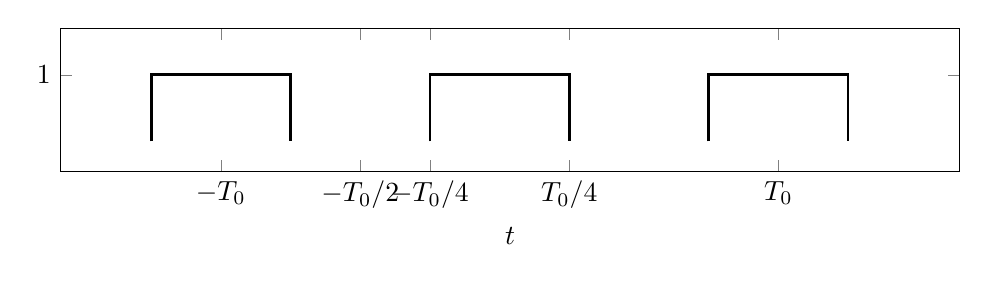
\begin{tikzpicture}
    \begin{axis}[width=13cm, height=3.4cm, xmin=-6.3, xmax=6.6, ymin=-0.45, ymax=1.7,
        xtick={-4,-2,-1,1,4}, xticklabels={$-T_0$,$-T_0/2$,$-T_0/4$,$T_0/4$,$T_0$}, ytick={1}, xlabel={$t$}]
      \addplot[black, line width=1pt] coordinates {(-5,0) (-5,1) (-3,1) (-3,0)};
      \addplot[black, line width=1pt] coordinates {(-1,0) (-1,1) (1,1) (1,0)};
      \addplot[black, line width=1pt] coordinates {(3,0) (3,1) (5,1) (5,0)};
    \end{axis}
  \end{tikzpicture}
\end{center}
\[ a_0=\frac{1}{2},\quad a_n=\frac{2}{\pi n}\sin\left(\frac{n\pi}{2}\right),\quad b_n=0 \]

Burdan geçir
\begin{align*}
a_n &= \frac{2}{T_0}\int_{-T_0/4}^{T_0/4}1\cdot\cos(n\omega_0 t)\,dt=\frac{2}{T_0}\left.\frac{\sin(n\omega_0 t)}{n\omega_0}\right|_{-T_0/4}^{T_0/4} \\
&= \frac{2}{n\underbrace{\omega_0 T_0}_{2\pi}}\underbrace{\left[\sin\left(n\omega_0\frac{T_0}{4}\right)-\sin\left(-n\omega_0\frac{T_0}{4}\right)\right]}_{2\sin\left(n\omega_0\frac{T_0}{4}\right)} \\
&= \frac{2}{\pi n}\sin\left(\frac{n\pi}{2}\right)
\end{align*}

\sayfa{7}
\sekilnotu[7]{Periyodik dikdörtgen darbe katarı grafiği: yatay eksen $t$, düşey eksende $1$ işaretli; genliği $1$ ve genişliği $\tau$ olan darbeler (kırmızı çift yönlü okla $-\tau/2$ ile $\tau/2$ arası gösterilmiş). Merkez darbe $[-\tau/2,\tau/2]$ aralığında, diğer darbeler $-T_0$ ve $T_0$ etrafında ortalı; eksende $-T_0$, $-T_0/2$, $-\tau/2$, $\tau/2$, $T_0/2$, $T_0$ işaretli.}

Ödev olarak ispatlayınız
\[ a_0=\frac{\tau}{T_0}\,,\qquad a_n=\frac{2}{\pi n}\sin\left(n\omega_0\frac{\tau}{2}\right)\,,\qquad b_n=0 \]

\sayfa{8}
\section{Bipolar square wave (Çift kutuplu kare dalga)}

\sekilnotu[8]{Çift kutuplu kare dalga grafiği: düşey eksen $x_b(t)$, yatay eksen $t$. Orijin etrafında ve $\pm T_0$ etrafında ortalı pozitif seviyeli darbeler, aralarında ($\pm T_0/2$ etrafında) negatif seviyeli kısımlar; eksende $-T_0$, $-T_0/2$, $T_0/2$, $T_0$ işaretli.}

\begin{align*}
x_b(t) &= 2x(t)-1 = 2\left[x(t)-\frac{1}{2}\right] \\
x_b(t) &= \frac{4}{\pi}\left[\cos(\omega_0 t)-\frac{1}{3}\cos(3\omega_0 t)+\frac{1}{5}\cos(5\omega_0 t)-\frac{1}{7}\cos(7\omega_0 t)+\cdots\right]
\end{align*}

\begin{ornek}
Dürtü treni (Impulse train) \\
$x(t)=s_{T_0}(t)=\displaystyle\sum_{n=-\infty}^{\infty}\delta(t-nT_0)$
\end{ornek}

\sekilnotu[8]{Dürtü treni: düşey eksen $x(t)$, yatay eksende $-2T_0$, $-T_0$, $0$, $T_0$, $2T_0$ noktalarında yukarı yönlü dürtüler (oklar); $-T_0/2$ ve $T_0/2$ noktalarında kesikli düşey çizgiler.}

\[ a_0=\frac{1}{T_0}\int_{T_0}x(t)\,dt=\frac{1}{T_0}\underbrace{\int_{-T_0/2}^{T_0/2}\underbrace{x(t)}_{\delta(t)}\,dt}_{1}=\frac{1}{T_0} \]

\formulkutu{\int_a^b f(t)\,\delta(t-t_0)\,dt=\begin{cases} f(t_0), & a<t_0<b \\ 0, & \text{diğer}\end{cases}}

\[ a_n=\frac{2}{T_0}\int_{-T_0/2}^{T_0/2}\underbrace{x(t)}_{\delta(t-0)}\underbrace{\cos(n\omega_0 t)}_{\cos(n\omega_0\cdot 0)=1}\,dt=\frac{2}{T_0} \]

$x(t)$ çift , $b_n=0$

\begin{align*}
x(t) &= \underbrace{\frac{1}{T_0}}_{a_0=c_0}+\sum_{n=1}^{\infty}\underbrace{\frac{2}{T_0}}_{a_n=c_n}\cos(n\omega_0 t) \\
&= \frac{1}{T_0}\left[1+2\sum_{n=1}^{\infty}\cos(n\omega_0 t)\right]
\end{align*}

\[ c_0=\frac{1}{T_0}\,,\quad c_n=\frac{2}{T_0}\,,\qquad \theta_n=0 \]

\sayfa{9}
\sekilnotu[9]{Tek taraflı spektrum: düşey eksen $c_n$ ($1/T_0$ ve $2/T_0$ seviyeleri işaretli), yatay eksen $nf_0$ ($0$, $f_0$, $2f_0$, $3f_0$ işaretli); $0$'da yüksekliği $1/T_0$, $f_0$, $2f_0$, $3f_0$'da yüksekliği $2/T_0$ olan kırmızı çubuklar.}

\subsection{Üstel FS açılımı}
\begin{align*}
x_n &= \frac{1}{T_0}\int_{T_0}x(t)e^{-jn\omega_0 t}\,dt \\
&= \frac{1}{T_0}\int_{-T_0/2}^{T_0/2}\underset{0}{\delta(t)}\,\underbrace{e^{-jn\omega_0 t}}_{f(t)}\,dt=\frac{1}{T_0}
\end{align*}
\begin{align*}
x(t) &= \sum_{n=-\infty}^{\infty}x_n e^{jn\omega_0 t}=\frac{1}{T_0}\sum_{n=-\infty}^{\infty}e^{jn\omega_0 t} \\
x(t) &= s_{T_0}(t)=\sum_{n=-\infty}^{\infty}\delta(t-nT_0)=\frac{1}{T_0}\sum_{n=-\infty}^{\infty}e^{jn\omega_0 t}
\end{align*}

\[ x_n=\frac{1}{T_0}\,,\qquad |x_n|=\frac{1}{T_0}\,,\qquad \theta_n=0 \]

\sekilnotu[9]{Çift taraflı spektrum: düşey eksen $x_n$ ($1/T_0$ işaretli), yatay eksen $nf_0$ ($-3f_0$, $-2f_0$, $-f_0$, $0$, $f_0$, $2f_0$, $3f_0$ işaretli); her noktada yüksekliği $1/T_0$ olan kırmızı çubuklar.}

\begin{ornek}
\sekilnotu[9]{Periyodik dikdörtgen darbe katarı: düşey eksen $x(t)$, merkez darbenin yüksekliği $A$; merkez darbe $-\tau/2$ ile $\tau/2$ arasında, diğer darbeler $\pm T_0$ etrafında ortalı; eksende $-T_0$, $-T_0/2$, $-\tau/2$, $\tau/2$, $T_0/2$, $T_0$ işaretli.}
\end{ornek}

\subsection{Üstel FS açılımı}
\begin{align*}
x_n &= \frac{1}{T_0}\int_{T_0}x(t)e^{-jn\omega_0 t}\,dt=\frac{1}{T_0}\int_{-T_0/2}^{T_0/2}x(t)e^{-jn\omega_0 t}\,dt \\
&= \frac{1}{T_0}\int_{-\tau/2}^{\tau/2}Ae^{-jn\omega_0 t}\,dt=\frac{A}{T_0}\left.\frac{e^{-jn\omega_0 t}}{-jn\omega_0}\right|_{-\tau/2}^{\tau/2} \\
&= -\frac{A}{jn\omega_0T_0}\left[e^{-jn\omega_0\frac{\tau}{2}}-e^{+jn\omega_0\frac{\tau}{2}}\right]=\frac{A}{n\pi}\sin\left(n\omega_0\frac{\tau}{2}\right)
\end{align*}

\sayfa{10}
\[ x_n=\frac{A}{\pi n}\sin\left(n\,2\pi f_0\frac{\tau}{2}\right)=\frac{A}{\pi n}\,\underbrace{\frac{\sin(n\pi f_0\tau)}{\pi n f_0\tau}}_{\mathrm{sinc}(nf_0\tau)}\cdot\,\pi n f_0\tau \]

\formulkutu{x_n=Af_0\tau\,\mathrm{sinc}(nf_0\tau)}

\[ x(t)=\sum_{n=-\infty}^{\infty}x_n e^{jn\omega_0 t}=\sum_{n=-\infty}^{\infty}\underbrace{Af_0\tau\,\mathrm{sinc}(nf_0\tau)}_{x_n}\cdot e^{jn\omega_0 t} \]

\[ \frac{T_0}{4}<\tau<\frac{T_0}{3}\ \rightarrow\ 3f_0<\frac{1}{\tau}<4f_0 \quad\text{aralığında olsun} \]

\sekilnotu[10]{$|x_n|$ grafiği: düşey eksen $|x_n|$, yatay eksen $nf_0$ ($0$, $f_0$, $2f_0$, $3f_0$, $4f_0$, $5f_0$, $6f_0$ işaretli; $3f_0$ ile $4f_0$ arasında $1/\tau$, sağda $2/\tau$ işaretli). Kırmızı çubuklar: $0$'da $Af_0\tau$, $f_0$'da $Af_0\tau\,|\mathrm{sinc}(f_0\tau)|$, $2f_0$'da $Af_0\tau\,|\mathrm{sinc}(2f_0\tau)|$, $3f_0$'da daha küçük; pembe kesikli $|\mathrm{sinc}|$ zarfı $1/\tau$'da sıfıra iniyor, $1/\tau$ ile $2/\tau$ arasında küçük bir yan lob yapıyor.}

\sekilnotu[10]{Faz grafiği: düşey eksen ($\pi$ ve $-\pi$ işaretli), yatay eksen $nf_0$ ($-6f_0,\dots,6f_0$ işaretli). Kırmızı çubuklar: $-6f_0$, $-5f_0$, $-4f_0$'da $+\pi$ yüksekliğinde; $4f_0$, $5f_0$, $6f_0$'da $-\pi$ derinliğinde; $0$ ile $4f_0$ arasında $-\pi$ seviyesinde kesikli çizgi. Pembe ok, üstteki grafikteki $1/\tau$ noktasından bu grafiğe iniyor.}

\[ -1=e^{-j\pi}=\underbrace{\cos\pi}_{-1}-j\underbrace{\sin\pi}_{0} \]

\subsection{Ödev}
\sekilnotu[10]{Blok diyagram: giriş oku $\rightarrow$ kutu ``$h(t)$'' $\rightarrow$ çıkış oku.}
\[ x(t)=\sum_n x_n e^{jn\omega_0 t} \qquad\qquad y(t)=\sum_n y_n e^{jn\omega_0 t} \]
\begin{align*}
y_n &= x_n H(nf_0) \\
H(f) &= \int_{-\infty}^{+\infty}h(t)\,e^{-j2\pi f t}\,dt
\end{align*}

$\ast$ Example 2.2.6

\sayfa{11}
\sekilnotu[11]{Bu sayfa basılı materyal içeriyor (ör. ders slaytı); dijitalleştirilmedi.}

\[ a_0=0\,,\qquad a_n=\frac{4}{\pi n}\sin\left(n\omega_0\frac{\tau}{2}\right) \]
\[ T_0=10^{-5}\,,\qquad \omega_0=\frac{2\pi}{T_0}=\frac{2\pi}{10^{-5}}=2\pi\,10^5\,,\qquad \tau=\frac{T_0}{2} \]
\begin{align*}
a_n &= \frac{4}{\pi n}\sin\left(n\,\frac{2\pi}{T_0}\cdot\frac{T_0}{4}\right) \\
&= \frac{4}{\pi n}\sin\left(\frac{n\pi}{2}\right)
\end{align*}
\[ b_n=0 \]
\[ x(t)=a_0+\sum_{n=1}^{\infty}\left[a_n\cos(n\omega_0 t)\right]+b_n\sin(n\omega_0 t) \]
\[ \sum_{n=1}^{\infty}\frac{4}{\pi n}\sin\left(\frac{n\pi}{2}\right)\cos\left(n\,2\pi\,10^5 t\right) \]

\end{document}
